\section{Implementace}
V předchozí kapitole jsme diskutovali matematickou úvahu o třídách a jejich skupinách (SubClasses), kde jsme stanovili tři klíčové podmínky: úplnost, disjunkci a podmnožinovou strukturu. V této kapitole se zaměříme na implementaci těchto matematických principů do třídního a databázového modelu. Zároveň se pokusíme najít nejefektivnější řešení, které zajistí plnou konzistenci dat v databázi.

\subsection{Třídní Model}

Třídní model zahrnuje několik hlavních entit: \texttt{Class}, \texttt{SubClass}, \texttt{Student} a \texttt{StudentAssignment}. Model \texttt{Class} reprezentuje třídu jako celek, model \texttt{SubClass} reprezentuje skupiny v rámci třídy, model \texttt{Student} reprezentuje jednotlivé žáky a model \texttt{StudentAssignment} zaznamenává přiřazení žáků k třídám a skupinám.

\subsubsection*{Class}

\texttt{Class} obsahuje informace o třídě, jako jsou identifikátor třídy, označení třídy, prefix, data platnosti, kmenovou učebnu a třídního učitele. 

V této implementaci není speciálně řešena změna třídního učitele nebo kmenové učebny během školního roku. Při změně je třeba ukončit validitu staré třídy a založit novou se stejným názvem. Dojte tedy k duplikování všech vazeb žáků, tříd, skupin a rozvrhů. Tyto případy jsou zcela výjimečné a tedy není třeba situaci řešit komplikovaněji.

\subsubsection*{SubClass}

\texttt{SubClass} reprezentuje skupiny žáků v rámci třídy. Každá skupina má své vlastní identifikační číslo, název a odkaz na třídu, ke které patří. SubClass může existovat pouze v kontextu třídy, což znamená, že každá SubClass musí být vždy přiřazena konkrétní třídě.

\subsubsection*{Student}

\texttt{Student} obsahuje informace o jednotlivých žácích, jako jsou identifikační číslo, uživatelské jméno, jméno a příjmení.

\subsubsection*{StudentAssignment}

\texttt{StudentAssignment} zaznamenává přiřazení žáků k třídám a skupinám. Obsahuje odkazy na žáky, třídy a skupiny, ke kterým jsou přiřazeni. Klíčovým prvkem tohoto modelu je zajištění trvanlivosti přiřazení, tedy schopnost zaznamenávat změny přiřazení žáků v průběhu roku. 

V průběhu školního roku mohou nastat různé změny, které vyžadují aktualizaci přiřazení žáků. Tyto změny mohou zahrnovat mnoho faktorů a ty nejčastější z nich jsou vyjmenovány níže. Trvanlivost přiřazení umožňuje udržovat historický záznam o všech těchto změnách, což je nezbytné pro správu.

\textbf{Problémy a důvody pro trvanlivost:}

\begin{itemize}
    \item \textbf{Přechody mezi třídami}: Žáci mohou být během školního roku přeřazeni do jiné třídy z různých důvodů, jako jsou změny nálad v třídním kolektivu nebo přestup žáka mezi obory.
    \item \textbf{Změny ve složení skupin}: V závislosti na specifických potřebách výuky mohou být žáci přeřazeni mezi různými skupinami. Například při výuce jazyků může být potřeba změnit složení skupin kvůli homogenizaci, nebo naopak heterogenizaci skupiny, čimž v závislosti na potřebách jednotlivých žáků lze docílit zefektivnění výuky.
\end{itemize}

Model \texttt{StudentAssignment} musí být schopen zaznamenávat všechny tyto změny, aby bylo možné udržovat konzistentní a aktuální přehled o přiřazení žáků. Tento model tedy umožňuje sledování přiřazení žáků k třídám a skupinám v určitém časovém období a zajišťuje, že historické změny jsou správně zaznamenány.

\textbf{Schopnosti modelu:}

\begin{itemize}
    \item \textbf{Referenční integrita}: Každý záznam o přiřazení musí odkazovat na platné záznamy ve třídách a skupinách.
    \item \textbf{Flexibilita přiřazení}: Umožňuje přiřazení žáka buď přímo do třídy nebo do specifické skupiny.
    \item \textbf{Trvanlivost}: Udržuje historické záznamy o přiřazení, které umožňují sledovat změny v průběhu školního roku.
\end{itemize}

Tímto způsobem model \texttt{StudentAssignment} nejen zajišťuje aktuálnost a konzistenci dat, ale také poskytuje cenné historické informace, které mohou být využity pro analýzu a zlepšení vzdělávacího procesu.

\begin{figure}[H]
    \centering
    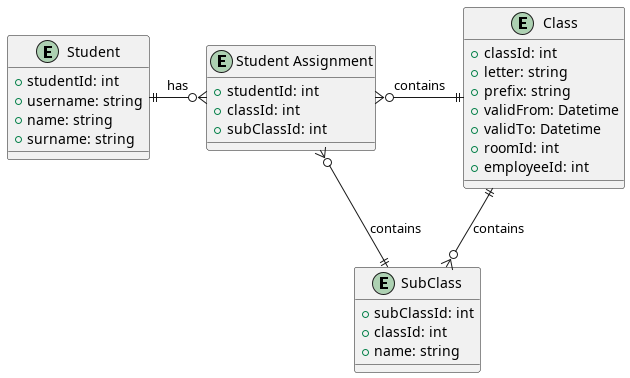
\includegraphics[width=.8\textwidth]{cd-student-assignment.png}
    \caption{Model tříd žákovských skupin}
    \label{fig:cd-student-assignment}
 \end{figure}

\subsection{Databázový Model}

Databázový model musí zajistit, že všechny podmínky úplnosti, disjunkce a podmnožinové struktury jsou dodrženy. Toho lze dosáhnout pomocí správného nastavení cizích klíčů, unikátních omezení a triggerů.

\subsubsection*{Úplnost}

Úplnost zajišťuje, že každá třída je pokryta skupinami tak, aby žádný žák nezůstal nezařazen v dané kategorii (tzn. dělení na poloviny, třetiny, dívky a chlapce). V backendové části zajistíme, že všechny skupiny dohromady pokrývají celou třídu. To můžeme kontrolovat při každém přiřazení žáka do skupiny. Je nezbytné, aby všechny skupiny dané kategorie třídy byly disjunktní a jejich sjednocení tvořilo celou třídu.

\subsubsection*{Disjunkce}

Disjunkci zajistíme na úrovni databáze pomocí unikátních omezení. Každý žák může patřit pouze do jedné skupiny určitého typu v dané třídě. To lze implementovat pomocí unikátních indexů nebo pomocí aplikační logiky, která před přiřazením žáka do skupiny provede potřebné kontroly.

\subsubsection*{Podmnožinová struktura}

Podmnožinovou strukturu zajistíme pomocí cizích klíčů a referenční integrity. Každá skupina musí odkazovat na existující třídu a každé přiřazení žáka do skupiny musí odkazovat na existujícího žáka, třídu a skupinu.

\subsection{Validace dat v aplikační logice}

Validace dat je důležitým aspektem jakéhokoliv robustního informačního systému. V tomto návrhu  systému zajišťuje validace dat konzistenci a integritu uložených informací. Níže jsou popsány validátory použité v aplikační logice.

\subsubsection*{Úvod do validace dat}

Validace dat je proces ověřování, zda vstupní data splňují stanovené požadavky a pravidla. Tato pravidla mohou zahrnovat různé aspekty, jako je formát, rozsah, konzistence a vztahy mezi jednotlivými datovými poli. Ve školním systému je validace dat implementována na úrovni aplikační logiky. To zajišťuje, že pouze správně formátovaná a platná data jsou ukládána do databáze.

V této aplikaci je použito několik validátorů, které kontrolují různé aspekty vstupních dat. Každý validátor je navržen tak, aby ověřil konkrétní sadu pravidel a zajistil, že data jsou konzistentní a správná.

\subsubsection*{Validátor dat třídy (\texttt{validateClassDates})}

Validátor \texttt{validateClassDates} je zodpovědný za ověření, zda datum začátku (\texttt{validFrom}) třídy je dříve než datum konce (\texttt{validTo}). Zajišťuje, že žádná třída nemůže mít začátek po svém konci, což by bylo nelogické a mohlo by vést k chybám při dalších operacích.

\begin{lstlisting}[title=Kód validátoru dat třídy]
function validateClassDates(instance: Class) {
    if (new Date(instance.validFrom) > new Date(instance.validTo)) {
        throw new Error('validFrom must be less than validTo');
    }
}
\end{lstlisting}

\subsubsection*{Validátor unikátnosti názvu třídy (\texttt{validateClassName})}

Validátor \texttt{validateClassName} ověřuje, že jméno třídy je unikátní v daném období platnosti. Tím je zajištěno, že nemůže existovat více tříd se stejným jménem v tomtéž období. Tím validátor předchází duplicitě názvů tříd, což by mohlo vést ke zmatkům a chybám v rozvrhu a přiřazení studentů.

\begin{lstlisting}[title=Kód validátoru unikátnosti názvu třídy]
async function validateClassName(instance: Class) {
    const existingClass = await Class.findOne({
        where: {
            name: instance.name,
            validFrom: { [Op.lte]: instance.validTo },
            validTo: { [Op.gte]: instance.validFrom }
        }
    });

    if (existingClass) {
        throw new Error('Class name already exists in the given period');
    }
}
\end{lstlisting}

\subsubsection*{Validátor časových intervalů tříd (\texttt{validateClassInterval})}

Validátor \texttt{validateClassInterval} zajišťuje, že nově vytvářená nebo aktualizovaná třída nemá časový interval, který by se překrýval s jinou třídou se stejným jménem, místností nebo učitelem. Tím zajišťuje, že třídy nebudou mít překrývající se časové intervaly, což by mohlo způsobit problémy s plánováním.

\newpage
\begin{lstlisting}[title=Kód validátoru časových intervalů tříd]
async function validateClassInterval(instance: Class) {
    const existingClass = await Class.findOne({
        where: {
          name: instance.name,
          roomId: instance.roomId,
          employeeId: instance.employeeId,
          validFrom: { [Op.lte]: instance.validTo },
          validTo: { [Op.gte]: instance.validFrom },
          classId: { [Op.ne]: instance.classId }
        }
      });
    
      if (existingClass) {
        throw new Error('Class interval is overlapping with another class');
      }
}
\end{lstlisting}

\subsubsection*{Validátor existence učitele (\texttt{validateTeacherExistence})}

Validátor \texttt{validateTeacherExistence} kontroluje, zda zaměstnanec, který je přiřazen k třídě, skutečně existuje v databázi a je učitel. Tím je zajištěno, že nejsou přiřazováni neexistující učitelé nebo nepedagogičtí zaměstnanci.

\begin{lstlisting}[title=Kód validátoru existence učitele]
async function validateTeacherExistence(instance: Class) {
    const teacher = await Employee.findOne({
        where: { employeeId: instance.employeeId, isTeacher: true }
      });
    
      if (!teacher) {
        throw new Error('Teacher does not exist');
      }
}
\end{lstlisting}

\subsubsection*{Validátor rozvrhu učitele (\texttt{validateEmployeeSchedule})}

Validátor \texttt{validateEmployeeSchedule} zajišťuje, že učitel nemá přiřazen více tříd ve stejném časovém období. Tím zajišťuje konflikty v rozvrzích učitelů.

\newpage
\begin{lstlisting}[title=Kód validátoru rozvrhu učitele]
async function validateEmployeeSchedule(instance: Class) {
    const existingTeacher = await Class.findOne({
        where: {
            employeeId: instance.employeeId,
            validFrom: { [Op.lte]: instance.validTo },
            validTo: { [Op.gte]: instance.validFrom },
            classId: { [Op.ne]: instance.classId }
        }
    });

    if (conflictingClass) {
        throw new Error('Teacher is already assigned to another class in this period');
    }
}
\end{lstlisting}

\subsubsection*{Validátor existence místnosti (\texttt{validateRoomExistence})}

Podobně jako validátor existence učitele, validátor \texttt{validateRoomExistence} ověřuje, že místnost přiřazená k třídě existuje v databázi a je učebnou. Zajišťuje, že místnost není například kancelář.

\begin{lstlisting}[title=Kód validátoru existence místnosti]
async function validateRoomExistence(instance: Class) {
    const room = await Room.findOne({ 
        where: { 
            roomId: instance.roomId,
            type: 'classroom'
        } 
    });
    
    if (!room) {
        throw new Error('Room does not exist');
    }
}
\end{lstlisting}

\subsubsection*{Validátor rozvrhu místnosti (\texttt{validateRoomSchedule})}

Validátor \texttt{validateRoomSchedule} ověřuje, že místnost není přiřazena více třídám ve stejném časovém období. Tím je zajištěno, že místnost může být kmenovou učebnou a místnost není přiřazena k více třídám zároveň.

\newpage
\begin{lstlisting}[title=Kód validátoru rozvrhu místností]
async function validateRoomSchedule(instance: Class) {
    const existingRoom = await Class.findOne({
        where: {
          roomId: instance.roomId,
          validFrom: { [Op.lte]: instance.validTo },
          validTo: { [Op.gte]: instance.validFrom },
          classId: { [Op.ne]: instance.classId }
        }
    });
    
    if (existingRoom) {
        throw new Error(
          'Room is already assigned to another class within the validity period'
        );
    }
}
\end{lstlisting}

\subsection{Diskuse o efektivitě řešení}

Pro zajištění úplné konzistence dat v databázi je nutné implementovat následující mechanismy.

\subsubsection*{Validace na úrovni aplikace}

Při každém přiřazení žáka do skupiny zkontrolujeme, zda přiřazení splňuje podmínky úplnosti a disjunkce. Pokud podmínky nejsou splněny, přiřazení se neprovede a uživatel obdrží příslušnou chybovou zprávu. Aplikační logika bude muset zohlednit také případy, kdy se celá třída učí společně a není třeba přiřazovat žáky do skupin.

\subsubsection*{Unikátní omezení}

Na úrovni databáze zavedeme unikátní omezení, která zajistí, že každý žák může patřit pouze do jedné skupiny určitého typu v dané třídě. Tím zajistíme disjunkci dat.

\subsubsection*{Referenční integrita}

Pomocí cizích klíčů zajistíme, že každá skupina je podmnožinou existující třídy a každé přiřazení žáka odkazuje na existujícího žáka, třídu a skupinu. Tím zajistíme podmnožinovou strukturu.

Implementace výše uvedených mechanismů v kombinaci s aplikační logikou poskytuje robustní řešení pro správu tříd a jejich skupin. Validace na úrovni aplikace umožňuje flexibilitu a zajišťuje, že jsou splněny všechny kladené podmínky. Unikátní omezení a referenční integrita na úrovni databáze zajišťují konzistenci dat a minimalizují riziko chyb.

Tímto způsobem zajišťujeme:

\begin{itemize}
    \item \textbf{Úplnost}: Každá třída je kompletně pokryta skupinami a žádný žák nezůstane nezařazen.
    \item \textbf{Disjunkce}: Každý žák může být přiřazen pouze do jedné skupiny určitého typu v dané třídě.
    \item \textbf{Podmnožinová struktura}: Každá skupina je vždy podmnožinou konkrétní třídy, ke které patří.
\end{itemize}